% !TeX TXS-program:bibliography = txs:///bibtex
\documentclass{article}

%\usepackage[T1]{fontenc}
\usepackage[margin=1in]{geometry}
\usepackage{parskip}

\usepackage{tikz}
	\usetikzlibrary{arrows,positioning}
	\tikzset{dpadded/.style={rounded corners=2, inner sep=0.7em, draw, outer sep=0.3em, fill={black!50}, fill opacity=0.08, text opacity=1}}
	\tikzset{arr/.style={draw, ->, thick, shorten <=3pt, shorten >=3pt}}

\usepackage{mathtools,amssymb}
\usepackage{amsthm}
\usepackage{thmtools} % asmsymb must be loaded also.
	\theoremstyle{plain}
	\newtheorem{poss}{Possible Result}
	\theoremstyle{definition}
	\declaretheorem[name=Definition,qed=$\square$]{defn}
	\declaretheorem[name=Def,unnumbered,qed=$\square$]{defn*}
%	\declaretheorem*[name=Definition,qed=$\square$]{defn*}
	\declaretheorem[name=Example,qed=$\square$]{example}
	\theoremstyle{remark}
	\newtheorem*{remark}{Remark}
	
\usepackage{color}
\usepackage{enumitem}
\usepackage[colorlinks=true,linkcolor=blue]{hyperref}

\usepackage{framed}

\DeclarePairedDelimiterX{\bbr}[1]{[}{]}{\mspace{-3.5mu}\delimsize[#1\delimsize]\mspace{-3.5mu}}
\DeclareMathAlphabet{\mathdcal}{U}{dutchcal}{m}{n}
\DeclareMathAlphabet{\mathbdcal}{U}{dutchcal}{b}{n}
\newcommand{\dg}[1]{\mathbdcal{#1}}
\newcommand{\thickD}{I\mkern-8muD}
\DeclarePairedDelimiterX{\infdivx}[2]{(}{)}{#1\;\delimsize\|\;#2}
\newcommand{\kldiv}{\thickD\infdivx}

\newcommand\mat[1]{\mathbf{#1}}

\newcommand{\bp}[1][L]{\mat{p}_{\!_{#1}\!}}
\newcommand{\V}{\mathcal V}
\newcommand{\N}{\mathcal N}
\newcommand{\Ed}{\mathcal E}

\usepackage[noabbrev,nameinlink]{cleveref}
\crefname{example}{example}{examples}
\crefname{defn}{definition}{definitions}
\crefname{prop}{proposition}{propositions}
\crefname{constr}{construction}{constructions}
\crefname{fact}{fact}{facts}

\newlength\todolength
\setlength\todolength{\textwidth-5pt}

\newcommand{\todo}[1]{
%\textbf{$\smash{\Large\boldsymbol{[}}$
		\colorbox{red!60!black}{\parbox{\todolength}{\color{white}$\mathrlap{\textbf{todo}}${\hspace{0.12ex}}\textbf{todo}: #1}}
%	 \!\!\smash{$\Large\boldsymbol{]}$}\!}
}


\begin{document}
	\begin{center}
		\bf\Large July 6 Report: Databases
	\end{center}
	\medskip
	
	
	
%	\section{Queries}
	
	\section{Deterministic Databases}
	Recall Vardi's \cite{vardi} definition of a relational database:
	\begin{leftbar}	
	\begin{defn*}
		An (untyped) database is a tuple $(D, R_1, \ldots, R_k)$, where $D$ is a finite set, and for each $i$, we have $R_i \subseteq D^{a_i} = \prod_{j =1}^{a_i} D$ 
		%(equivalently to emphasize structural similarity with the definition below, $R_i \in 2^{D^{a_i}}$)
		for some \emph{arity} $a_i \in \mathbb N$. 
	\end{defn*}
	\end{leftbar}

	We alter the presentation and notation slightly, without changing the mathematical structure, so that can formally define $a$, and avoid possible future confusion with the numbered indices. 

	\begin{defn}
		An (untyped) database is a tuple $(D, I, a, \mathcal R)$, where $D$ is a finite set (the universal domain), $I$ is a finite index set, $a: I \to \mathbb N$ is the arity function (for each $i \in I$, $a_i$ is the \emph{arity} of the $i^{\text{th}}$ relation), and $\mathcal R = \{R_i\}_{i \in I}$ is a finite collection of relations on $D$, so that for each $i \in I$, we have $R_i \subseteq D^{a_i} = \prod_{j =1}^{a_i} D$.
		%(equivalently to emphasize structural similarity with the definition below, $R_i \in 2^{D^{a_i}}$)
	\end{defn}

 	We are actually interested in a \emph{typed} version, of which the former is a special case.
	
%	\begin{defn}
%		A (typed) database is a tuple $(\mathcal D, \tau, a, R_1, \ldots, R_k)$, where $\mathcal D$ is a collection of finite domains, where again $a_i \in \mathbb N$ is the arity, $\tau(i,j) \in \mathcal D$ is the type of the $j^{\text{th}}$ dimension of the relation $R_i$, and each $R_i \subseteq \prod_{j =1}^{a_i} \mathcal D_{\tau(i,j)} $.
%	\end{defn}
	\begin{defn}
		A (typed) database is a tuple $(\mathcal D, I, a, \tau, \mathcal R)$, where $\mathcal D$ is a collection of finite domains (the different types), again $a: I \to \mathbb N$ determines the arity, but now $\tau_i \in \mathcal D^{a_i}$ associates each relation with a length-$a_i$ vector of types. 
		%
		Concretely, for any $i \in I$, and any $j \in 1, \ldots a_i$, $\tau_{i,j} \in \mathcal D$ is the $j^{\text{th}}$ component of the relation $R_i$, so that 
	 	$R_i \subseteq \prod \tau_i = \prod_{j =1}^{a_i} \tau_{i,j}.$ 
	\end{defn}

	\begin{remark}
		The definition of an untyped database with underlying domain $D$ is clearly a special case of a typed database, where $\mathcal D := \{ D \}$, and each $\tau_{i,j} = D$. 
		In some sense, the two are equally expressive; by setting $D := \sqcup \mathcal D$ to be the disjoint union of each domain, any typed database on $\mathcal D$ is in particular an untyped database on $D$, since
		\[R_i \in 2^{\left\{\prod \tau_i\right\}} = 2^{\left\{\prod_{j =1}^{a_i} \tau_{i,j}\right\}} 
			\subseteq 2^{\left\{D^{a_i}\right\}} .\] 
		However, the definitions are not equivalent, and the typed version is more expressive, because it \emph{dis}-allows some instances, encoding type-level constraints. As we will see, this distinction is particularly important for us, because the types here correspond to different random variables. 
		
	\end{remark}
	
	\subsection{Database Schemas and PDGs}
	
	Generally, we think of a database as a collection of tables with keys, rows, and attributes; we will now connect this with PDGs
	
	\todo{Insert simple the examples I came up that worked like I had hoped}\\
	\todo{Connect this to the formalism above}
	
	We now turn to an example which clearly illustrates this use of a database schema (see \href{http://math.mit.edu/~dspivak/informatics/notes/unorganized/CTDB--spivakCurino.pdf}{this paper on unified basis of database formalism}, based on a category theory presentation which is very close to my categorical definition of a PDG, which to a first approximation, is: a diagram of the Markov category).
	
	\begin{example} \label{ex:dpt-emp}
		Suppose a business has multiple departments, and each department has two distinguished employees: the secretary, and the manager. 
		The directed multi-graph $\mathcal G$ below is a schema of the resulting database.
		\begin{center}
			$\mathcal G := (\N, \Ed) :=\qquad$
			\scalebox{0.8}{
			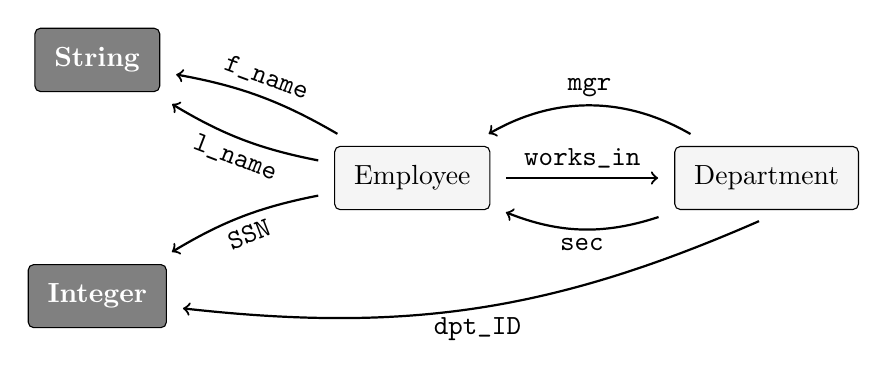
\begin{tikzpicture}[baseline]
				\node[dpadded] (emp) at (0,0) {Employee};
				\node[dpadded] (dpt) at (4.5,0) {Department};

				\node[dpadded, opacity=1, text=white] (str) at (-4,1.5) {\textbf{String}};
				\node[dpadded, opacity=1, text=white] (int) at (-4,-1.5) {\textbf{Integer}};
				
				\draw[arr] (dpt) to[bend left=20] node[below] {\texttt{sec}} (emp);
				\draw[arr] (dpt) to[bend right] node[above] {\texttt{mgr}} (emp)   ;
				
				\draw[arr] (emp) to node[above] {\texttt{works\char`_in}} (dpt) ;
				
				\draw[arr] (emp) to[bend right=10] node[above,sloped] {\texttt{f\char`_name}} (str);
				\draw[arr] (emp) to[bend left=10] node[below,sloped] {\texttt{l\char`_name}} (str);
				\draw[arr] (emp) to[bend right=10] node[below,sloped] {\texttt{SSN}} (int);
%				\draw[arr] (emp) to[bend right=10] node[above,sloped] {\texttt{salary}} (int);
				\draw[arr] (dpt.south) to[bend left=15] node[below] {\texttt{dpt\char`_ID}} (int);
			\end{tikzpicture}}
			\smallskip
		\end{center}
	
		First, the good news: this multigraph $\mathcal G = (\N, \Ed)$ can be used directly as the structure of a PDG. Better still, an instance of the database (that is, including table rows) can be be encoded in the other two components $(\V, \mat p)$ of a PDG; $\V$ associates each node $N \in \N$ with a finite set of values, and each edge $L: X \to Y$ with a deterministic function $\bp$ (which is, in particular, a degenerate cpd). In table form, one instance of the database schema above can be seen in the following two tables:
		
		\begin{center}
			\begin{tabular}{r|cc}
				\textbf{Department} & \texttt{sec} & \texttt{mgr} \\
				\hline
				Sales & Alice & Bob\\
				Marketing & Carl & Dora\\
			\end{tabular}
			\hspace{1cm}
			\begin{tabular}{l|llrl}
				\textbf{Employee} & \texttt{f\char`_name} & \texttt{l\char`_name} & \texttt{SSN} & \texttt{works\char`_in}\\
				\hline
				Alice & Allie & Smith & 4 & Sales\\
				Bob & Robert & Baker & 2 & Sales\\
				Carl & Carligo & Qi & 11 & Marketing\\
				Dora & Dora & Jargol & 33 & Marketing\\
			\end{tabular}
		\end{center}
		Each arrow gives a column of the table (the value of the variable corresponding to the arrow's target node).		
		In this way, a collection of tables determines both $\V$ and $\bp$. 	
	\end{example}

	\emph{Encoding} a database as a PDG is therefore straightforward and natural, but the story is not so simple. The semantics of joint distributions over values don't make a whole lot of sense. Recall that our ``possible worlds'' were joint settings of random variables: but here joint settings are tupples $(s,i,e,d)$ where $s$ is a string (which we have constrained to equal both the employee's first and last names)

	Perhaps even worse, for schemas like that in \Cref{ex:dpt-emp}, because each arrow is deterministic, if every distribution is given an infinitely bad score, unless all incoming arrows agree on the exact value (in \Cref{ex:dpt-emp} in particular, every cpd coming into the node ``String'' must have all mass on a  \texttt{l\char`_name}$=$\texttt{f\char`_name}).

	
	\begin{remark}
		A distribution over (emp, dept, arrow) makes sense to score (for a
		deterministic database, return prior on source, and corresponding posterior on
		target), but it is not clear that a joint distribution of this kind will contain
		exactly the right information. It is unsatisfying, for instance, that we have to
		weigh the probability of the "event" Department=Sales against that of the disjoint
		"event" Department=Marketing when clearly the two are co-existing departments.
	\end{remark}

\subsection{Possible Resolutions}
\todo{Not finished; because I ran out of time, but I've tried to make them readable to a third party, and a more concrete research plan, which may be worth commenting on.}

	Many of the immediate solutions of a certain class require us to clone variables, as would be done in a \href{https://en.wikipedia.org/wiki/Plate_notation}{plate notation}. 
	
	\begin{itemize}[nosep]
		\item Mark certain nodes as ``coppied'', so that effectively they are duplicated for every edge leading to them.
		\item Similarly, mark some arrows as ``duplicating''.
		\item Similarly, mark 2-cells as ``commuting'' or ``non-commuting''
		(in \Cref{ex:dpt-emp}, \texttt{f\char`_name}, \texttt{l\char`name} do not form a commutative triangle)
		\item Use \(\beta\)'s, to effectively isolate at only at a subset of edges at a time. This makes scores finite and we can restrict to interpret-able subsets, but does not. Such an approach would be complimented by a way of putting these pieces together to get a single score of the appropriate mental object, that agrees with our previous scoring function whenever it makes sense to apply.
		
		\item Have a heirarchy / poset, so that using a reference to a lower-level item duplicates it.
	\end{itemize}

	However, the compact description (made possible by independence of the clones) should be also easy to be scored compactly, without going through the intermediate ``compilation step'' of ``unstacking of plates'' to get a normal graphical model. Still, a difference in scores between the compressed model of this kind, and an unwound one, would demand a justification.
	
	
	We might also be able to simply extend our semantics so that it scores not only joint distributions, but also other, more general objects. Fortunately, the identity of a scoring function is contra-variant in is argument: because (distribution OR other proposition) is a weaker constraint than just (distribution), we might be able to naturally extend the scoring function we already have. In other words, it seems the nonsense is self-imposed: why insist on accepting only a distribution over joint variable settings, when joint variable settings do not even make sense as possible worlds?
	
	From this perspective, we should refocus our effort on:
	
	\begin{itemize}[nosep]
		\item Distributions over trees / polytrees / flows
		\item Distributions over paths
	\end{itemize}

	\subsection{Deterministic PDGs as Relational Databases}

	\section{Probabilistic Databases}
	\todo{Finish standard definitions from probabilistic database literature, collect some potentially useful theorems about them here as I read.}
	
	\begin{defn}
		A probabilistic database is a database in which either
		\begin{itemize}[nosep]
			\item Each tuple appears in a table with a given probability (specified to be independent-from-all-others probability, and given structurally as a special column of each table)
			\item The value of a tuple (if it exists) has uncertainty about its value.
		\end{itemize}
	\end{defn}
%	The two are related to the two presentations of sub-stochasticity; 
	

	
\end{document}